\documentclass[a4paper, 12pt]{article}

% packages
\usepackage{amssymb}
\usepackage[fleqn]{mathtools}
\usepackage{tikz}
\usepackage{enumerate}
\usepackage{bussproofs}
\usepackage{xcolor}
\usepackage[margin=1.3cm]{geometry}
\usepackage{logicproof}
\usepackage{diagbox}
\usepackage{listings}
\usepackage{graphicx}
\usepackage{lstautogobble}
\usepackage{hyperref}
\usepackage{multirow}
\usepackage{tipa}
\usepackage{pgfplots}

% tikz libraries
\usetikzlibrary{
    decorations.pathreplacing,
    arrows,
    shapes.gates.logic.US,
    circuits.logic.US,
    calc,
    automata,
    positioning,
    intersections
}

\pgfplotsset{compat=1.16}

\pgfmathdeclarefunction{gauss}{2}{%
  \pgfmathparse{1/(#2*sqrt(2*pi))*exp(-((x-#1)^2)/(2*#2^2))}%
}

\allowdisplaybreaks % allow environments to break
\setlength\parindent{0pt} % no indent

% shorthand for verbatim
% this clashes with logicproof, so maybe fix this at some point?
\catcode`~=\active
\def~#1~{\texttt{#1}}

% code listing
\lstdefinestyle{main}{
    numberstyle=\tiny,
    breaklines=true,
    showspaces=false,
    showstringspaces=false,
    tabsize=2,
    numbers=left,
    basicstyle=\ttfamily,
    columns=fixed,
    fontadjust=true,
    basewidth=0.5em,
    autogobble,
    xleftmargin=3.0ex,
    mathescape=true
}
\newcommand{\dollar}{\mbox{\textdollar}} %
\lstset{style=main}

% augmented matrix
\makeatletter
\renewcommand*\env@matrix[1][*\c@MaxMatrixCols c]{%
\hskip -\arraycolsep
\let\@ifnextchar\new@ifnextchar
\array{#1}}
\makeatother

% ceiling / floor
\DeclarePairedDelimiter{\ceil}{\lceil}{\rceil}
\DeclarePairedDelimiter{\floor}{\lfloor}{\rfloor}

% custom commands
\newcommand{\indefint}[2]{\int #1 \, \mathrm{d}#2}
\newcommand{\defint}[4]{\int_{#1}^{#2} #3 \, \mathrm{d}#4}
\newcommand{\pdif}[2]{\frac{\partial #1}{\partial #2}}
\newcommand{\dif}[2]{\frac{\mathrm{d}#1}{\mathrm{d}#2}}
\newcommand{\limit}[2]{\raisebox{0.5ex}{\scalebox{0.8}{$\displaystyle{\lim_{#1 \to #2}}$}}}
\newcommand{\limitsup}[2]{\raisebox{0.5ex}{\scalebox{0.8}{$\displaystyle{\limsup_{#1 \to #2}}$}}}
\newcommand{\summation}[2]{\sum\limits_{#1}^{#2}}
\newcommand{\product}[2]{\prod\limits_{#1}^{#2}}
\newcommand{\intbracket}[3]{\left[#3\right]_{#1}^{#2}}
\newcommand{\laplace}{\mathcal{L}}
\newcommand{\fourier}{\mathcal{F}}
\newcommand{\mat}[1]{\boldsymbol{#1}}
\renewcommand{\vec}[1]{\boldsymbol{#1}}
\newcommand{\rowt}[1]{\begin{bmatrix}
    #1
\end{bmatrix}^\top}
\DeclareMathOperator*{\argmax}{argmax}
\DeclareMathOperator*{\argmin}{argmin}

\newcommand{\lto}[0]{\leadsto\ }

\newcommand{\ulsmash}[1]{\underline{\smash{#1}}}

\newcommand{\powerset}[0]{\wp}
\renewcommand{\emptyset}[0]{\varnothing}

\makeatletter
\newsavebox{\@brx}
\newcommand{\llangle}[1][]{\savebox{\@brx}{\(\m@th{#1\langle}\)}%
  \mathopen{\copy\@brx\kern-0.5\wd\@brx\usebox{\@brx}}}
\newcommand{\rrangle}[1][]{\savebox{\@brx}{\(\m@th{#1\rangle}\)}%
  \mathclose{\copy\@brx\kern-0.5\wd\@brx\usebox{\@brx}}}
\makeatother
\newcommand{\lla}{\llangle}
\newcommand{\rra}{\rrangle}
\newcommand{\la}{\langle}
\newcommand{\ra}{\rangle}
\newcommand{\crnr}[1]{\text{\textopencorner} #1 \text{\textcorner}}
\newcommand{\bnfsep}[0]{\ |\ }
\newcommand{\concsep}[0]{\ ||\ }

\newcommand{\axiom}[1]{\AxiomC{#1}}
\newcommand{\unary}[1]{\UnaryInfC{#1}}
\newcommand{\binary}[1]{\BinaryInfC{#1}}
\newcommand{\trinary}[1]{\TrinaryInfC{#1}}
\newcommand{\quaternary}[1]{\QuaternaryInfC{#1}}
\newcommand{\quinary}[1]{\QuinaryInfC{#1}}
\newcommand{\dproof}[0]{\DisplayProof}
\newcommand{\llabel}[1]{\LeftLabel{\scriptsize #1}}
\newcommand{\rlabel}[1]{\RightLabel{\scriptsize #1}}

\newcommand{\ttbs}{\char`\\}
\newcommand{\lrbt}[0]{\ \bullet\ }

% colours
\newcommand{\violet}[1]{\textcolor{violet}{#1}}
\newcommand{\blue}[1]{\textcolor{blue}{#1}}
\newcommand{\red}[1]{\textcolor{red}{#1}}
\newcommand{\teal}[1]{\textcolor{teal}{#1}}

% reasoning proofs
\usepackage{ltablex}
\usepackage{environ}
\keepXColumns
\NewEnviron{reasoning}{
    \begin{tabularx}{\textwidth}{rlX}
        \BODY
    \end{tabularx}
}
\newcommand{\proofline}[3]{$(#1)$ & $#2$ & \hfill #3 \smallskip \\}
\newcommand{\proofarbitrary}[1]{& take arbitrary $#1$ \smallskip \\}
\newcommand{\prooftext}[1]{\multicolumn{3}{l}{#1} \smallskip \\}
\newcommand{\proofmath}[3]{$#1$ & = $#2$ & \hfill #3 \smallskip \\}
\newcommand{\prooftherefore}[1]{& $\therefore #1$ \smallskip \\}
\newcommand{\proofbc}[0]{\prooftext{\textbf{Base Case}}}
\newcommand{\proofis}[0]{\prooftext{\textbf{Inductive Step}}}

% ER diagrams
\newcommand{\nattribute}[4]{
    \node[draw, state, inner sep=0cm, minimum size=0.2cm, label=#3:{#4}] (#1) at (#2) {};
}
\newcommand{\mattribute}[4]{
    \node[draw, state, accepting, inner sep=0cm, minimum size=0.2cm, label=#3:{#4}] (#1) at (#2) {};
}
\newcommand{\dattribute}[4]{
    \node[draw, state, dashed, inner sep=0cm, minimum size=0.2cm, label=#3:{#4}] (#1) at (#2) {};
}
\newcommand{\entity}[3]{
    \node[] (#1-c) at (#2) {#3};
    \node[inner sep=0cm] (#1-l) at ($(#1-c) + (-1, 0)$) {};
    \node[inner sep=0cm] (#1-r) at ($(#1-c) + (1, 0)$) {};
    \node[inner sep=0cm] (#1-u) at ($(#1-c) + (0, 0.5)$) {};
    \node[inner sep=0cm] (#1-d) at ($(#1-c) + (0, -0.5)$) {};
    \draw
    ($(#1-c) + (-1, 0.5)$) -- ($(#1-c) + (1, 0.5)$) -- ($(#1-c) + (1, -0.5)$) -- ($(#1-c) + (-1, -0.5)$) -- cycle;
}
\newcommand{\relationship}[3]{
    \node[] (#1-c) at (#2) {#3};
    \node[inner sep=0cm] (#1-l) at ($(#1-c) + (-1, 0)$) {};
    \node[inner sep=0cm] (#1-r) at ($(#1-c) + (1, 0)$) {};
    \node[inner sep=0cm] (#1-u) at ($(#1-c) + (0, 1)$) {};
    \node[inner sep=0cm] (#1-d) at ($(#1-c) + (0, -1)$) {};
    \draw
    ($(#1-c) + (-1, 0)$) -- ($(#1-c) + (0, 1)$) -- ($(#1-c) + (1, 0)$) -- ($(#1-c) + (0, -1)$) -- cycle;
}

% AVL Trees
\newcommand{\avltri}[4]{
    \draw ($(#1)$) -- ($(#1) + #4*(0.5, -1)$) -- ($(#1) + #4*(-0.5, -1)$) -- cycle;
    \node at ($(#1) + #4*(0, -1) + (0, 0.5)$) {#3};
    \node at ($(#1) + #4*(0, -1) + (0, -0.5)$) {#2};
}

% RB Trees
\tikzset{rbtr/.style={inner sep=2pt, circle, draw=black, fill=red}}
\tikzset{rbtb/.style={inner sep=2pt, circle, draw=black, fill=black}}

% actual document
\begin{document}
    \section*{CO240 - Models of Computation \hfill Tutorial Sheets}
        \subsection*{Tutorial 1 - Expressions}
            \begin{enumerate}[1.]
                \itemsep0em
                \item
                    Consider the \textbf{big-step} operational semantics for the language \textit{SimpleExp} given in the lectures.
                    Find a number $n$ such that
                    \begin{center}
                        $(4 + 1) + (2 + 2) \Downarrow n$
                    \end{center}
                    Give the full derivation tree.
                    \begin{center}
                                    \axiom{}
                                \llabel{(B-NUM)}
                                \unary{$4 \Downarrow 4$}
                                    \axiom{}
                                \llabel{(B-NUM)}
                                \unary{$1 \Downarrow 1$}
                            \llabel{(B-ADD)}
                            \binary{$(4 + 1) \Downarrow 5$}
                                    \axiom{}
                                \llabel{(B-NUM)}
                                \unary{$2 \Downarrow 2$}
                                    \axiom{}
                                \llabel{(B-NUM)}
                                \unary{$2 \Downarrow 2$}
                            \llabel{(B-ADD)}
                            \binary{$(2 + 2) \Downarrow 2$}
                        \llabel{(B-ADD)}
                        \binary{$(4 + 1) + (2 + 2) \Downarrow 9$}
                        \dproof
                    \end{center}
                \item
                    The big-step operation semantics for \textit{SimpleExp} was only given for addition.
                    Extend it to include \textit{multiplication}.
                    Give a proof that $((3 + 2) \times (1 + 4)) \Downarrow 25$
                    \medskip

                    To do this, we need to add an additional rule as follows;
                    \begin{center}
                            \axiom{$E_1 \Downarrow n_1$}
                            \axiom{$E_2 \Downarrow n_2$}
                        \llabel{(B-MUL)}
                        \rlabel{$n_3 = n_1 \times n_2$}
                        \binary{$E_1 \times E_2 \Downarrow n_3$}
                        \dproof
                    \end{center}
                    Hence we can do the following;
                    \begin{center}
                                    \axiom{}
                                \llabel{(B-NUM)}
                                \unary{$3 \Downarrow 3$}
                                    \axiom{}
                                \llabel{(B-NUM)}
                                \unary{$2 \Downarrow 2$}
                            \llabel{(B-ADD)}
                            \binary{$(3 + 2) \Downarrow 5$}
                                    \axiom{}
                                \llabel{(B-NUM)}
                                \unary{$1 \Downarrow 1$}
                                    \axiom{}
                                \llabel{(B-NUM)}
                                \unary{$4 \Downarrow 4$}
                            \llabel{(B-ADD)}
                            \binary{$(1 + 4) \Downarrow 5$}
                        \llabel{(B-MUL)}
                        \binary{$((3 + 2) \times (1 + 4)) \Downarrow 25$}
                        \dproof
                    \end{center}
                \item
                    Extend the \textbf{big-step} semantics further to include \textit{subtraction}.
                    Remember that the numbers in the syntax of the language are $0, 1, 2, \dots$ (no negative numbers).
                    \smallskip

                    How is an expression such as $(3 - 7)$ handled in your semantics?
                    Have you made any arbitrary decisions about this?
                    If so, what other options were available?
                    \medskip

                    Note that this question has multiple valid options; we can either introduce a ~NaN~ concept, representing an "invalid" operation, which has to be propagated in all rules, or we could have it be some value.
                    The latter can lead to ambiguity, because if we had $(3 - 7) \Downarrow 0$, and also $(4 - 7) \Downarrow 0$, we may unexpected results.
                \item Recall the \textbf{small-step} operational semantics of \textit{SimpleExp}.
                    \begin{enumerate}[(a)]
                        \itemsep0em
                        \item
                            Give the full derivation of the first step of evaluation of $((1 + 2) + (4 + 3))$ - give the derivation tree of the step (for some expression $E$);
                            \begin{center}
                                $((1 + 2) + (4 + 3)) \to E$
                            \end{center}
                            For the first step, we have the following;
                            \begin{center}
                                        \axiom{}
                                    \llabel{(S-ADD)}
                                    \unary{$(1 + 2) \to 3$}
                                \llabel{(S-LEFT)}
                                \unary{$((1 + 2) + (4 + 3)) \to (3 + (4 + 3))$}
                                \dproof
                            \end{center}
                        \item
                            Write down all the steps of evaluation needed to reduce the above expression to 10.
                            Give the full derivation for each of these steps.
                            \medskip

                            Note that the \textbf{evaluation path} is;
                            \begin{center}
                                $((1 + 2) + (4 + 3)) \to (3 + (4 + 3)) \to (3 + 7) \to 10$
                            \end{center}
                            The derivation tree for each step is as follows;
                            \begin{center}
                                        \axiom{}
                                    \llabel{(S-ADD)}
                                    \unary{$(4 + 3) \to 7$}
                                \llabel{(S-RIGHT)}
                                \unary{$(3 + (4 + 3)) \to (3 + 7)$}
                                \dproof
                            \end{center}
                            Followed by;
                            \begin{center}
                                    \axiom{}
                                \llabel{(S-ADD)}
                                \unary{$(3 + 7) \to 10$}
                                \dproof
                            \end{center}
                    \end{enumerate}
                \item Here is the abstract syntax for a simple language \textit{Bool} of boolean expressions:
                    \begin{center}
                        $B \in \textit{Bool} ::= ~true~ \bnfsep ~false~ \bnfsep B \& B \bnfsep \neg B \bnfsep ~if ~ B ~ then ~ B ~ else ~ B$
                    \end{center}
                    Intuitively, every expression evaluates to either ~true~ or ~false~.
                    \begin{enumerate}[(a)]
                        \itemsep0em
                        \item Give a \textbf{small-step} operational semantics for \textit{Bool}.
                            \begin{center}
                                    \axiom{$B_1 \to B_1^\prime$}
                                \unary{$B_1 \& B_2 \to B_1^\prime \& B_2$}
                                \dproof
                                \medskip

                                    \axiom{$B_2 \to B_2^\prime$}
                                \unary{$~true~ \& B_2 \to ~true~ \& B_2^\prime$}
                                \dproof
                                \medskip

                                    \axiom{$B_2 \to B_2^\prime$}
                                \unary{$~false~ \& B_2 \to ~false~ \& B_2^\prime$}
                                \dproof
                                \medskip

                                    \axiom{}
                                \unary{$~true~ \& ~true~ \to ~true~$}
                                \dproof
                                \medskip

                                    \axiom{}
                                \unary{$~true~ \& ~false~ \to ~false~$}
                                \dproof
                                \medskip

                                    \axiom{}
                                \unary{$~false~ \& ~true~ \to ~false~$}
                                \dproof
                                \medskip

                                    \axiom{}
                                \unary{$~false~ \& ~false~ \to ~false~$}
                                \dproof
                                \medskip

                                    \axiom{$B \to B^\prime$}
                                \unary{$\neg B \to \neg B^\prime$}
                                \dproof
                                \medskip

                                    \axiom{}
                                \unary{$\neg ~true~ \to ~false~$}
                                \dproof
                                \medskip

                                    \axiom{}
                                \unary{$\neg ~false~ \to ~true~$}
                                \dproof
                                \medskip

                                    \axiom{$B_1 \to B_1^\prime$}
                                \unary{$~if ~ B_1 ~ then ~ B_2 ~ else ~ B_3$}
                                \dproof
                                \medskip

                                    \axiom{}
                                \unary{$~if true then ~ B_2 ~ else ~ B_3 \to B_2$}
                                \dproof
                                \medskip

                                    \axiom{}
                                \unary{$~if false then ~ B_2 ~ else ~ B_3 \to B_3$}
                                \dproof
                            \end{center}
                            Note that these are all evaluated right-to-left.
                        \item Write down all the steps of evaluation needed to reduce the following expression to a result:
                            \begin{align*}
                                & \neg (~if ~ (~false~ \& ~true~) ~ then ~ (~if true then ~ (~false~ \& ~true~) ~ else false~) ~ else ~ \neg ~true~) \\
                                \to\ & \neg (~if false then ~ (~if true then ~ (~false~ \& ~true~) ~ else false~) ~ else ~ \neg ~true~) \\
                                \to\ & \neg (\neg ~true~) \\
                                \to\ & \neg ~false~ \\
                                \to\ & ~true~
                            \end{align*}
                    \end{enumerate}
                \item
                    The syntax of \textit{SimpleExp} is extended with a new operator $?$, as follows;
                    \begin{center}
                        $E \in \textit{SimpleExp} ::= \dots \bnfsep (E ? E)$
                    \end{center}
                    This operator allows the implementation to choose to give the result of $E_1$, or $E_2$, when given $E_1 ? E_2$.
                    \begin{enumerate}[(a)]
                        \itemsep0em
                        \item Extend the \textbf{big-step} operational semantics with rules for $?$ that capture this meaning.
                            \begin{center}
                                \hfill
                                    \axiom{$E_1 \Downarrow n_1$}
                                \llabel{(B-CHOICE-1)}
                                \unary{$E_1 ? E_2 \Downarrow n_1$}
                                \dproof
                                \hfill
                                    \axiom{$E_2 \Downarrow n_2$}
                                \llabel{(B-CHOICE-2)}
                                \unary{$E_1 ? E_2 \Downarrow n_2$}
                                \dproof
                                \hfill \phantom{}
                            \end{center}
                        \item For what values of $n$ does $(0 ? 1) + (2 ? 3) \Downarrow n$?
                            \begin{center}
                                            \axiom{}
                                        \llabel{(B-NUM)}
                                        \unary{$0 \Downarrow 0$}
                                    \llabel{(B-CHOICE-1)}
                                    \unary{$(0 ? 1) \Downarrow 0$}
                                            \axiom{}
                                        \llabel{(B-NUM)}
                                        \unary{$2 \Downarrow 2$}
                                    \llabel{(B-CHOICE-1)}
                                    \unary{$(2 ? 3) \Downarrow 2$}
                                \llabel{(B-ADD)}
                                \binary{$(0 ? 1) + (2 ? 3) \Downarrow 2$}
                                \dproof
                                \medskip

                                            \axiom{}
                                        \llabel{(B-NUM)}
                                        \unary{$0 \Downarrow 0$}
                                    \llabel{(B-CHOICE-1)}
                                    \unary{$(0 ? 1) \Downarrow 0$}
                                            \axiom{}
                                        \llabel{(B-NUM)}
                                        \unary{$3 \Downarrow 3$}
                                    \llabel{(B-CHOICE-2)}
                                    \unary{$(2 ? 3) \Downarrow 3$}
                                \llabel{(B-ADD)}
                                \binary{$(0 ? 1) + (2 ? 3) \Downarrow 3$}
                                \dproof
                                \medskip

                                            \axiom{}
                                        \llabel{(B-NUM)}
                                        \unary{$1 \Downarrow 1$}
                                    \llabel{(B-CHOICE-2)}
                                    \unary{$(0 ? 1) \Downarrow 1$}
                                            \axiom{}
                                        \llabel{(B-NUM)}
                                        \unary{$2 \Downarrow 2$}
                                    \llabel{(B-CHOICE-1)}
                                    \unary{$(2 ? 3) \Downarrow 2$}
                                \llabel{(B-ADD)}
                                \binary{$(0 ? 1) + (2 ? 3) \Downarrow 3$}
                                \dproof
                                \medskip

                                            \axiom{}
                                        \llabel{(B-NUM)}
                                        \unary{$1 \Downarrow 1$}
                                    \llabel{(B-CHOICE-2)}
                                    \unary{$(0 ? 1) \Downarrow 1$}
                                            \axiom{}
                                        \llabel{(B-NUM)}
                                        \unary{$3 \Downarrow 3$}
                                    \llabel{(B-CHOICE-2)}
                                    \unary{$(2 ? 3) \Downarrow 3$}
                                \llabel{(B-ADD)}
                                \binary{$(0 ? 1) + (2 ? 3) \Downarrow 4$}
                                \dproof
                            \end{center}
                        \item
                            Is the semantics deterministic?
                            Is it total?
                            \medskip

                            It is not deterministic as we have $0 ? 1 \Downarrow 0$, as well as $0 ? 1 \Downarrow 1$ - but $0 \neq 1$.
                            It is total as it is applies to every expression (for something to be total, we need some number $n$ for every expression $E$ such that $E \Downarrow n$).
                    \end{enumerate}
                \item
                    \begin{enumerate}[(a)]
                        \itemsep0em
                        \item Extend the \textbf{small-step} semantics for \textit{SimpleExp} to handle the $?$ operator by adding appropriate derivation rules for $\to$.
                            \begin{center}
                                \hfill
                                    \axiom{}
                                \llabel{(S-CHOICE-1)}
                                \unary{$E_1 ? E_2 \to E_1$}
                                \dproof
                                \hfill
                                    \axiom{}
                                \llabel{(S-CHOICE-2)}
                                \unary{$E_1 ? E_2 \to E_2$}
                                \dproof
                                \hfill \phantom{}
                            \end{center}
                        \item Give all possible derivations of the first step of evaluation of $(0 ? 1) + (2 ? 3)$.
                            \begin{center}
                                \hfill
                                        \axiom{}
                                    \llabel{(S-CHOICE-1)}
                                    \unary{$0 ? 1 \to 0$}
                                \llabel{(S-LEFT)}
                                \unary{$(0 ? 1) + (2 ? 3) \to 0 + (2 ? 3)$}
                                \dproof
                                \hfill
                                        \axiom{}
                                    \llabel{(S-CHOICE-2)}
                                    \unary{$0 ? 1 \to 1$}
                                \llabel{(S-LEFT)}
                                \unary{$(0 ? 1) + (2 ? 3) \to 1 + (2 ? 3)$}
                                \dproof
                                \hfill \phantom{}
                            \end{center}
                        \item Give all of the possible evaluation paths for $(0 ? 1) + (2 ? 3)$.
                            \begin{center}
                                $(0 ? 1) + (2 ? 3) \to 0 + (2 ? 3) \to 0 + 2 \to 2$

                                $(0 ? 1) + (2 ? 3) \to 0 + (2 ? 3) \to 0 + 3 \to 3$

                                $(0 ? 1) + (2 ? 3) \to 1 + (2 ? 3) \to 1 + 2 \to 3$

                                $(0 ? 1) + (2 ? 3) \to 1 + (2 ? 3) \to 1 + 3 \to 4$
                            \end{center}
                        \item Is the semantics confluent?
                            \medskip

                            We've shown $(0 ? 1) + (2 ? 3) \to^* 2$ and also $(0 ? 1) + (2 ? 3) \to^* 3$.
                            Therefore, for the semantics to be confluent, there must be some $E^\prime$ such that $2 \to^* E^\prime$ and $3 \to^* E^\prime$ - however, since they are both in normal forms, they can only evaluate to themselves.
                            $2 \neq 3$, hence it is not confluent.
                        \item Is the semantics normalising?
                            \medskip

                            Yes, there are no infinite sequences of expressions, hence any evaluation path will eventually reach a normal form.
                    \end{enumerate}
                \item Suppose that instead of the \textit{SimpleExp} small-step rule {\scriptsize (S-RIGHT)}, we had the following;
                    \begin{center}
                            \axiom{$E_2 \to E_2^\prime$}
                        \llabel{(S-RIGHT$^\prime$)}
                        \unary{$(E_1 + E_2) \to (E_1 + E_2^\prime)$}
                        \dproof
                    \end{center}
                    \begin{enumerate}[(a)]
                        \itemsep0em
                        \item Given an evaluation path using the {\scriptsize S-RIGHT} rule, is it also an evaluation path using the {\scriptsize S-RIGHT$^\prime$} rule?
                            \medskip

                            Yes, as the original rule constrained $E_1$ to be in a normal form, but the new rule doesn't.
                            This means that the new rule covers all the cases of the original rule.
                        \item Find an expression that has an evaluation path using the {\scriptsize S-RIGHT$^\prime$} rule that it did not have with the {\scriptsize S-RIGHT} rule.
                            \begin{center}
                                $(0 + 1) + (2 + 3) \to (0 + 1) + 5 \to 1 + 5 \to 6$
                            \end{center}
                        \item Is $\to$ deterministic?
                            \medskip

                            No, starting with $(0 + 1) + (2 + 3)$, we can go to either $1 + (2 + 3)$ {\scriptsize S-LEFT}, or $(0 + 1) + 5$ with {\scriptsize S-RIGHT$^\prime$} - however the two expressions are not equal.
                        \item Is $\to$ confluent?
                            \medskip

                            Yes, the rule allows for different evaluation order, but doesn't change the result of the evaluation.
                    \end{enumerate}
            \end{enumerate}
        \subsection*{Tutorial 2 - State}
            \begin{enumerate}[1.]
                \itemsep0em
                \item
                    Consider the small-step operation semantics of the language \textit{While}.
                    Write down all of the evaluation steps of the program $(z := x; x := y); y := z$, with the initial state $s = (x \mapsto 5, y \mapsto 7)$.
                    Give the full derivation tree for the first step in this evaluation.
                    \begin{center}
                                        \axiom{}
                                    \llabel{(W-EXP.VAR)}
                                    \unary{$\la x, (x \mapsto 5, y \mapsto 7) \ra \to_e \la 5, (x \mapsto 5, y \mapsto 7) \ra$}
                                \llabel{(W-ASS.EXP)}
                                \unary{$\la z := x, (x \mapsto 5, y \mapsto 7) \ra \to_c \la z := 5, (x \mapsto 5, y \mapsto 7) \ra$}
                            \llabel{(W-SEQ.LEFT)}
                            \unary{$\la z := x; x := y, (x \mapsto 5, y \mapsto 7) \ra \to_c \la z := 5; x := y, (x \mapsto 5, y \mapsto 7) \ra$}
                        \llabel{(W-SEQ.LEFT)}
                        \unary{$\la (z := x; x := y); y := z, (x \mapsto 5, y \mapsto 7) \ra \to_c \la (z := 5; x := y); y := z, (x \mapsto 5, y \mapsto 7) \ra$}
                        \dproof
                    \end{center}
                    All of the steps are as follows;
                    \begin{align*}
                        & \la (z := x; x := y); y := z, (x \mapsto 5, y \mapsto 7) \ra \\
                        \to_c\ & \la (z := 5; x := y); y := z, (x \mapsto 5, y \mapsto 7) \ra \\
                        \to_c\ & \la (~skip~; x := y); y := z, (x \mapsto 5, y \mapsto 7, z \mapsto 5) \ra \\
                        \to_c\ & \la x := y; y := z, (x \mapsto 5, y \mapsto 7, z \mapsto 5) \ra \\
                        \to_c\ & \la x := 7; y := z, (x \mapsto 5, y \mapsto 7, z \mapsto 5) \ra \\
                        \to_c\ & \la ~skip~; y := z, (x \mapsto 7, y \mapsto 7, z \mapsto 5) \ra \\
                        \to_c\ & \la y := z, (x \mapsto 7, y \mapsto 7, z \mapsto 5) \ra \\
                        \to_c\ & \la y := 5, (x \mapsto 7, y \mapsto 7, z \mapsto 5) \ra \\
                        \to_c\ & \la ~skip~, (x \mapsto 7, y \mapsto 5, z \mapsto 5) \ra
                    \end{align*}
                \item
                    Consider the small-step operational semantics of the language \textit{While}.
                    Write down all of the evaluation steps of the program (given the initial state $s = (x \mapsto 1)$)
                    \begin{center}
                        $\violet{(\text{let } W =)}\ ~while ~ x < 4 ~ do ~ x := x + 2$
                    \end{center}
                    Give full derivation trees for the first four steps.
                    \begin{center}
                            \axiom{}
                        \llabel{1}
                        \unary{$\la ~while ~ x < 4 ~ do ~ x := x + 2, (x \mapsto 1) \ra \to_c\ \la ~if ~ x < 4 ~ then ~ (x := x + 2; W) ~ else skip~, (x \mapsto 1) \ra$}
                        \dproof
                        \medskip

                                    \axiom{}
                                \llabel{(W-EXP.VAR)}
                                \unary{$\la x, (x \mapsto 1) \ra \to_e \la 1, (x \mapsto 1) \ra$}
                            \llabel{(W-BEXP.LEFT)}
                            \unary{$\la x < 4, (x \mapsto 1) \ra \to_b \la 1 < 4, (x \mapsto 1) \ra$}
                        \llabel{2}
                        \unary{$\la ~while ~ x < 4 ~ do ~ x := x + 2, (x \mapsto 1) \ra \to_c\ \la ~if ~ 1 < 4 ~ then ~ (x := x + 2; W) ~ else skip~, (x \mapsto 1) \ra$}
                        \dproof
                        \medskip

                                \axiom{}
                            \llabel{(W-BEXP.LT)}
                            \unary{$\la 1 < 4, (x \mapsto 1) \ra \to_b \la ~true~, (x \mapsto 1) \ra$}
                        \llabel{2}
                        \unary{$\la ~while ~ x < 4 ~ do ~ x := x + 2, (x \mapsto 1) \ra \to_c\ \la ~if true then ~ (x := x + 2; W) ~ else skip~, (x \mapsto 1) \ra$}
                        \dproof
                        \medskip

                            \axiom{}
                        \llabel{(W-COND.TRUE)}
                        \unary{$\la ~if true then ~ (x := x + 2; W) ~ else skip~, (x \mapsto 1) \ra \to_c\ \la x := x + 2; W, (x \mapsto 1) \ra$}
                        \dproof
                    \end{center}
                    Note that rule 1 is {\scriptsize (W-WHILE)}, and rule 2 is {\scriptsize (W-COND.BEXP)}.
                    The full evaluation path is as follows;
                    \begin{align*}
                        & \la ~while ~ x < 4 ~ do ~ x := x + 2, (x \mapsto 1) \ra \\
                        \to_c\ & \la ~if ~ x < 4 ~ then ~ (x := x + 2; W) ~ else skip~, (x \mapsto 1) \ra \\
                        \to_c\ & \la ~if ~ 1 < 4 ~ then ~ (x := x + 2; W) ~ else skip~, (x \mapsto 1) \ra \\
                        \to_c\ & \la ~if true then ~ (x := x + 2; W) ~ else skip~, (x \mapsto 1) \ra \\
                        \to_c\ & \la x := x + 2; W, (x \mapsto 1) \ra \\
                        \to_c\ & \la x := 1 + 2; W, (x \mapsto 1) \ra \\
                        \to_c\ & \la x := 3; W, (x \mapsto 1) \ra \\
                        \to_c\ & \la ~skip~; W, (x \mapsto 3) \ra \\
                        \to_c\ & \la ~while ~ x < 4 ~ do ~ x := x + 2, (x \mapsto 3) \ra \\
                        \to_c\ & \la ~if ~ x < 4 ~ then ~ (x := x + 2; W) ~ else skip~, (x \mapsto 3) \ra \\
                        \to_c\ & \la ~if ~ 3 < 4 ~ then ~ (x := x + 2; W) ~ else skip~, (x \mapsto 3) \ra \\
                        \to_c\ & \la ~if true then ~ (x := x + 2; W) ~ else skip~, (x \mapsto 3) \ra \\
                        \to_c\ & \la x := x + 2; W, (x \mapsto 3) \ra \\
                        \to_c\ & \la x := 3 + 2; W, (x \mapsto 3) \ra \\
                        \to_c\ & \la x := 5; W, (x \mapsto 3) \ra \\
                        \to_c\ & \la ~skip~; W, (x \mapsto 5) \ra \\
                        \to_c\ & \la ~while ~ x < 4 ~ do ~ x := x + 2, (x \mapsto 5) \ra \\
                        \to_c\ & \la ~if ~ x < 4 ~ then ~ (x := x + 2; W) ~ else skip~, (x \mapsto 5) \ra \\
                        \to_c\ & \la ~if ~ 5 < 4 ~ then ~ (x := x + 2; W) ~ else skip~, (x \mapsto 5) \ra \\
                        \to_c\ & \la ~if false then ~ (x := x + 2; W) ~ else skip~, (x \mapsto 5) \ra \\
                        \to_c\ & \la ~skip~, (x \mapsto 5) \ra
                    \end{align*}
                \item
                    Consider adding the increment expression $x++$ to the language \textit{While}.
                    The expression returns the value of the variable (only applied to variables) $x$ and then updates the value of $x$ to be one greater than the old value; its semantics is given by the following rule:
                    \begin{center}
                            \axiom{}
                        \llabel{(W-EXP.PP)}
                        \rlabel{$s(x) = n, n^\prime = n + 1$}
                        \unary{$\la x++, s \ra \to_e \la n, s[x \mapsto n^\prime] \ra$}
                        \dproof
                    \end{center}
                    \begin{enumerate}[(a)]
                        \itemsep0em
                        \item Give the full execution path for the program $x := (x++) + (x++)$ from the initial state $(x \mapsto 2)$.
                            \begin{align*}
                                & \la x := (x++) + (x++), (x \mapsto 2) \ra \\
                                \to_c\ & \la x := 2 + (x++), (x \mapsto 3) \ra \\
                                \to_c\ & \la x := 2 + 3, (x \mapsto 4) \ra \\
                                \to_c\ & \la x := 5, (x \mapsto 4) \ra \\
                                \to_c\ & \la ~skip~, (x \mapsto 5) \ra
                            \end{align*}
                        \item Given an operational semantics rule for $++x$, which increments $x$ and then returns the result.
                            \begin{center}
                                    \axiom{}
                                \llabel{(W-EXP.PP)}
                                \rlabel{$s(x) = n, n^\prime = n + 1$}
                                \unary{$\la ++x, s \ra \to_e \la n^\prime, s[x \mapsto n^\prime] \ra$}
                                \dproof
                            \end{center}
                    \end{enumerate}
                \item
                    Consider what happens if we add a 'side-effecting expression' of the form
                    \begin{center}
                        $~do ~ C ~ return ~ E$
                    \end{center}
                    This runs first runs the command $C$, and returns the value of $E$.
                    \begin{center}
                        \hfill
                            \axiom{$\la C, s \ra \to_c \la C^\prime, s^\prime \ra$}
                        \unary{$\la ~do ~ C ~ return ~ E, s \ra \to_e \la ~do ~ C^\prime ~ return ~ E, s^\prime \ra$}
                        \dproof
                        \hfill
                            \axiom{}
                        \unary{$\la ~do skip return ~ E, s \ra \to_e \la E, s \ra$}
                        \dproof
                        \hfill \phantom{}
                    \end{center}
                \item
                    Consider the \textit{While} language extend with parallel composition of commands: $C \concsep C$.
                    The semantics of parallel composition is given by interleaving the execution steps of the two composed commands in an arbitrary fashion.
                    This is expressed formally as;
                    \begin{center}
                        \hfill
                            \axiom{$\la C_1, s \ra \to_c \la C_1^\prime, s^\prime \ra$}
                        \unary{$\la C_1 \concsep C_2, s \ra \to_c \la C_1^\prime \concsep C_2, s^\prime \ra$}
                        \dproof
                        \hfill
                            \axiom{$\la C_2, s \ra \to_c \la C_2^\prime, s^\prime \ra$}
                        \unary{$\la C_1 \concsep C_2, s \ra \to_c \la C_1 \concsep C_2^\prime, s^\prime \ra$}
                        \dproof
                        \hfill
                            \axiom{}
                        \unary{$\la ~skip~ \concsep ~skip~, s \ra \to_c \la ~skip~, s \ra$}
                        \dproof
                        \hfill \phantom{}
                    \end{center}
                    \begin{enumerate}[(a)]
                        \itemsep0em
                        \item
                            Consider the command $(x := 1) \concsep (x := 2; x := (x + 2))$, run with initial state $s = (x \mapsto 0)$.
                            How many possible final values for $x$ does this command have?
                            \medskip

                            There are 3 possible values; 1, 3, or 4.
                        \item How many different evaluation paths exist for obtaining the final value 4?
                            \medskip

                            3 paths.
                            I really can't be bothered to type out all of the steps.
                            The point is the operation $x := x + 2$ is not atomic; even if we have obtained $x := 4$, we can execute $x := 1$, and then still obtain a state with $x \mapsto 4$, if the former is executed at the end.
                        \item
                            A useful operation in concurrency is atomic compare-and-swap.
                            This operation is added to the \textit{While} language in the form of a new boolean expression $~CAS~(x, E, E)$.
                            To execute the operation $~CAS~(x, E_1, E_2)$, first $E_1$ and then $E_2$ are evaluated to numbers $n_1$ and $n_2$ in the usual way.
                            Then, \textbf{in a single step}, the operation compares the value of variable $x$ with $n_1$; if the values are equal, it updates the value of $x$ to be number $n_2$ and returns ~true~, otherwise, it simply returns ~false~.
                            Extend the operational semantics with rules for ~CAS~ that implement this behaviour.
                            \begin{center}
                                    \axiom{$\la E_1, s \ra \to_e \la E_1^\prime, s^\prime \ra$}
                                \unary{$\la ~CAS~(x, E_1, E_2), s \ra \to_b \la ~CAS~(x, E_1^\prime, E_2), s^\prime \ra$}
                                \dproof
                                \medskip

                                    \axiom{$\la E_2, s \ra \to_e \la E_2^\prime, s^\prime \ra$}
                                \unary{$\la ~CAS~(x, n_1, E_2), s \ra \to_b \la ~CAS~(x, n_1, E_2^\prime), s^\prime \ra$}
                                \dproof
                                \medskip

                                    \axiom{}
                                \rlabel{$s(x) = n_1$}
                                \unary{$\la ~CAS~(x, n_1, n_2), s \ra \to_b \la ~true~, s[x \mapsto n_2] \ra$}
                                \dproof
                                \medskip

                                    \axiom{}
                                \rlabel{$s(x) \neq n_1$}
                                \unary{$\la ~CAS~(x, n_1, n_2), s \ra \to_b \la ~false~, s \ra$}
                                \dproof
                            \end{center}
                    \end{enumerate}
                \item
                    Suppose that $\la C_1; C_2, s \ra \to_c^* \la C_2, s^\prime \ra$.
                    Show that it is not necessarily the case that $\la C_1, s \ra \to_c^* \la ~skip~, s^\prime \ra$.
                    \medskip

                    Let there be a state $s^{\prime\prime} \neq s^\prime$, where $\la C_1, s \ra \to_c^* \la ~skip~, s^{\prime\prime} \ra$.
                    For $\la C_1; C_2, s \ra \to_c^* \la C_2, s^\prime \ra$, we can find $C_2$ such that $\la C_2, s^{\prime\prime} \ra \to_c^* \la C_2, s^\prime \ra$.
                    From here, we see that our foal is to find $C_2$ as something that evaluates to itself, but in a different state (hence a loop).
                    \begin{align*}
                        C_1 & = ~skip~ \\
                        C_2 & = ~while true do ~ x := 1 \\
                        s & = (x \mapsto 0)
                    \end{align*}
                    Executing this we have;
                    \begin{align*}
                        & \la ~while true do ~ x := 1, (x \mapsto 0) \ra \\
                        \to_c\ & \la ~if true then ~ x := 1; C_2 ~ else skip~, (x \mapsto 0) \ra \\
                        \to_c\ & \la x := 1; C_2, (x \mapsto 0) \ra \\
                        \to_c\ & \la ~skip~; C_2, (x \mapsto 1) \ra \\
                        \to_c\ & \la C_2, (x \mapsto 1) \ra
                    \end{align*}
            \end{enumerate}
        \subsection*{Tutorial 3 - Induction}
            \begin{enumerate}[1.]
                \itemsep0em
                \item s
                    Binary trees are a commonly used data structure.
                    Roughly, a binary tree is either a single leaf node, or a branch node which has two subtrees.
                    The set of binary trees can be defined formally by the following grammar;
                    \begin{center}
                        $~bTree~ ::= ~Node~ \bnfsep ~Branch~(~bTree~, ~bTree~)$
                    \end{center}
                    \begin{enumerate}[(a)]
                        \itemsep0em
                        \item Draw pictures of the following binary trees;
                            \begin{itemize}
                                \itemsep0em
                                \item ~Node~
                                    \begin{center}
                                        
\begin{tikzpicture}
                                            \node[rbtb] at (0, 0) {};
                                        \end{tikzpicture}
                                    \end{center}
                                \item $~Branch~(T_1, T_2)$
                                    \begin{center}
                                        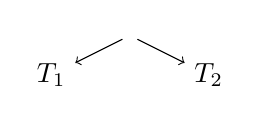
\begin{tikzpicture}
                                            \node[inner sep=2pt, circle] (o) at (0, 0) {};
                                            \node (ol) at (-1, -0.5) {$T_1$};
                                            \node (or) at (1, -0.5) {$T_2$};
                                            \draw
                                            (o) edge[->] (ol)
                                            (o) edge[->] (or);
                                        \end{tikzpicture}
                                    \end{center}
                                \item $~Branch~(~Node~, ~Node~)$
                                    \begin{center}
                                        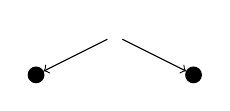
\begin{tikzpicture}
                                            \node[inner sep=2pt, circle] (o) at (0, 0) {};
                                            \node[rbtb] (ol) at (-1, -0.5) {};
                                            \node[rbtb] (or) at (1, -0.5) {};
                                            \draw
                                            (o) edge[->] (ol)
                                            (o) edge[->] (or);
                                        \end{tikzpicture}
                                    \end{center}
                                \item $~Branch~(~Node~, ~Branch~(~Node~, ~Node~))$
                                    \begin{center}
                                        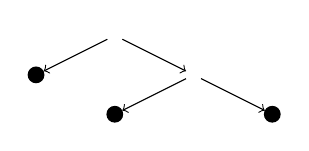
\begin{tikzpicture}
                                            \node[inner sep=2pt, circle] (o) at (0, 0) {};
                                            \node[rbtb] (ol) at (-1, -0.5) {};
                                            \node[inner sep=2pt, circle] (or) at (1, -0.5) {};
                                            \node[rbtb] (orl) at (0, -1) {};
                                            \node[rbtb] (orr) at (2, -1) {};
                                            \draw
                                            (o) edge[->] (ol)
                                            (o) edge[->] (or)
                                            (or) edge[->] (orl)
                                            (or) edge[->] (orr);
                                        \end{tikzpicture}
                                    \end{center}
                            \end{itemize}
                        \item d
                            We define th function ~leaves~ which takes a binary tree as an argument and returns the number of leaf nodes, given by ~Node~, in a tree, and similarly ~branches~, which counts the number of ~Branch~(\_, \_) nodes in a tree:
                            \begin{align*}
                                ~leaves~(~Node~) & = 1 \\
                                ~leaves~(~Branch~(T_1, T_2)) & = ~leaves~(T_1) + ~leaves~(T_2) \\
                                ~branches~(~Node~) & = 0 \\
                                ~branches~(~Branch~(T_1, T_2)) & = ~branches~(T_1) + ~branches~(T_2) + 1
                            \end{align*}
                            Prove by induction on the structure of trees, that for any tree $T$;
                            \begin{center}
                                $~leaves~(T) = ~branches~(T) + 1$
                            \end{center}
                            This trivially checks out for the base case, as we have
                            \begin{center}
                                $~leaves~(~Node~) = 1 = 0 + 1 = ~branches~(~Node~) + 1$
                            \end{center}
                            For the inductive step, let $T = ~Branch~(T_1, T_2)$, and assume that this holds for $T_1$ and $T_2$;
                            \begin{align*}
                                ~leaves~(T_1) & = ~branches~(T_1) + 1 & \text{inductive hypothesis} \\
                                ~leaves~(T_2) & = ~branches~(T_2) + 1 & \text{inductive hypothesis} \\
                                ~leaves~(T) & = ~leaves~(T_1) + ~leaves~(T_2) & \text{by def. of ~leaves~} \\
                                & = ~branches~(T_1) + 1 + ~branches~(T_2) + 1 & \text{by substitution} \\
                                & = ~branches~(~Branch~(T_1, T_2)) + 1 & \text{by def. of ~branches~} \\
                                & = ~branches~(T) + 1 & \blacksquare
                            \end{align*}
                    \end{enumerate}
                \item
                    Recall the \textbf{big-step} operational semantics for simple expressions $E$.
                    Prove by structural induction on the structure of expressions that, for every $E$, there is some number $n$ such that $E \Downarrow n$.
                    \begin{center}
                        $E \in \textit{SimpleExp} ::= n \bnfsep E + E$
                    \end{center}
                    Trivially, for the base case, $n \Downarrow n$.
                    For the case where we have $E = E_1 + E_2$, assume this holds for $E_1$ and $E_2$, such that $E_1 \Downarrow n_1$ and $E_2 \Downarrow n_2$.
                    Then $E_1 + E_2 \Downarrow n_3$, by {\scriptsize (B-ADD)}, where $n_3 = n_1 + n_2$.
                \setcounter{enumi}{3}
                \item
                    Recall the \textbf{small-step} operational semantics for simple expressions.
                    Prove, by induction on the structure of simple expressions, that for every expression $E$, either $E = n$ for some number $n$, or $E \to E^\prime$ for some expression $E^\prime$.
                    \medskip

                    We can first formalise the property as $P(E) \equiv (\exists n.\ E = n) \lor (\exists E^\prime.\ E \to E^\prime)$.

                    Trivially, the base case $P(n)$ (where $n$ is an arbitrary number), holds as $n$ is the number itself.
                    The inductive step has the following inductive hypothesis;
                    \begin{enumerate}[(1)]
                        \itemsep0em
                        \item $\violet{(\exists n_1.\ E_1 = n_1)} \lor \teal{(\exists E_1^\prime.\ E_1 \to E_1^\prime)}$
                        \item $\red{(\exists n_2.\ E_2 = n_2)} \lor \blue{(\exists E_2^\prime.\ E_2 \to E_2^\prime)}$
                    \end{enumerate}
                    For $E = E_1 + E_2$, we can look at the following cases;
                    \begin{itemize}
                        \itemsep0em
                        \item $\violet{E_1 = n_1}$ and $\red{E_2 = n_2}$ \hfill
                                \axiom{}
                            \llabel{(S-ADD)}
                            \rlabel{$n_3 = \violet{n_1} + \red{n_2}$}
                            \unary{$\violet{n_1} + \red{n_2} \to n_3$}
                            \dproof
                        \item $\violet{E_1 = n_1}$ and $\blue{E_2 \to E_2^\prime}$ \hfill
                                \axiom{$\blue{E_2 \to E_2^\prime}$}
                            \llabel{(S-RIGHT)}
                            \unary{$\violet{n_1} + \blue{E_2} \to \violet{n_1} + \blue{E_2^\prime}$}
                            \dproof
                        \item $\teal{E_1 \to E_1^\prime}$ \hfill
                            \axiom{$\teal{E_1 \to E_1^\prime}$}
                        \llabel{(S-LEFT)}
                        \unary{$\teal{E_1} + E_2 \to \teal{E_1^\prime} + E_2$}
                        \dproof
                    \end{itemize}
                \item Recall the \textbf{small-step} operational semantics for simple expressions.
                    \begin{enumerate}[(a)]
                        \itemsep0em
                        \item By induction on the structure of simple expressions, define a function $~ops~ : \textit{SimpleExp} \to \mathbb{N}$ that gives the number of operators in an expression.
                            \begin{align*}
                                ~ops~(n) & = 0 \\
                                ~ops~(E_1 + E_2) & = ~ops~(E_1) + ~ops~(E_2) + 1
                            \end{align*}
                        \item By induction on the structure of simple expressions, prove that for all simple expressions, $E$, $E^\prime$, with $E \to E^\prime$, $~ops~(E) > ~ops~(E^\prime)$.
                            \medskip

                            Since the proofs for $+$ and $\times$ are pretty much identical, only the former will be written out.
                            Let us first write this property as $P(E) \equiv \forall E^\prime.\ E \to E^\prime \Rightarrow ~ops~(E) > ~ops~(E^\prime)$.
                            This holds trivially for the base case, as there is no $E^\prime$ such that $n \to E^\prime$ for arbitrary $n$.
                            \medskip

                            For the inductive step, let $E = E_1 + E_2$, hence the inductive hypothesis is;
                            \begin{enumerate}[(1)]
                                \itemsep0em
                                \item $P(E_1) \equiv \forall E_1^\prime.\ E_1 \to E_1^\prime \Rightarrow ~ops~(E_1) > ~ops~(E_1^\prime)$
                                \item $P(E_2) \equiv \forall E_2^\prime.\ E_2 \to E_2^\prime \Rightarrow ~ops~(E_2) > ~ops~(E_2^\prime)$
                            \end{enumerate}
                            Hence we can use the definition of ~ops~ as follows, with three cases corresponding to the rules and axioms;
                            \begin{align*}
                                \intertext{
                                        \axiom{$E_1 \to E_1^\prime$}
                                    \llabel{(S-LEFT)}
                                    \unary{$E_1 + E_2 \to E_1^\prime + E_2$}
                                    \dproof
                                    \hfill
                                }
                                ~ops~(E) & = ~ops~(E_1 + E_2) \\
                                & = ~ops~(E_1) + ~ops~(E_2) + 1 & \text{by def. of ~ops~} \\
                                & > ~ops~(E_1^\prime) + ~ops~(E_2) + 1 & \text{by inductive hypothesis (1)} \\
                                & = ~ops~(E_1^\prime + E_2) & \text{by def. of ~ops~} \\
                                & = ~ops~(E^\prime)
                                \intertext{
                                        \axiom{$E_2 \to E_2^\prime$}
                                    \llabel{(S-RIGHT)}
                                    \unary{$n_1 + E_2 \to n_1 + E_2^\prime$}
                                    \dproof
                                    \hfill
                                    $E_1 = n_1$
                                }
                                ~ops~(E) & = ~ops~(n_1 + E_2) \\
                                & = ~ops~(n_1) + ~ops~(E_2) + 1 & \text{by def. of ~ops~} \\
                                & > ~ops~(n_1) + ~ops~(E_2^\prime) + 1 & \text{by inductive hypothesis (2)} \\
                                & = ~ops~(n_1 + E_2^\prime) & \text{by def. of ~ops~} \\
                                & = ~ops~(E^\prime)
                                \intertext{
                                        \axiom{}
                                    \llabel{(S-ADD)}
                                    \rlabel{$n_3 = n_1 + n_2$}
                                    \unary{$n_1 + n_2 \to n_3$}
                                    \dproof
                                    \hfill
                                    $E_1 = n_1$ and $E_2 = n_2$
                                }
                                ~ops~(E) & = ~ops~(n_1 + n_2) \\
                                & = ~ops~(n_1) + ~ops~(n_2) + 1 & \text{by def. of ~ops~} \\
                                & = 1 & \text{by def. of ~ops~} \\
                                & > 0 \\
                                & = ~ops~(n_3) & \text{by def. of ~ops~} \\
                                & = ~ops~(E^\prime)
                            \end{align*}
                            Hence it follows for all $E$.
                        \item Hence or otherwise, prove that $\to$ is normalising.
                            \medskip

                            As each evaluation causes ~ops~ to decrease, we know it will eventually terminate as ~ops~ will reach 0.
                            When it does reach 0, it will be a number, hence it must eventually reach this normal form.
                    \end{enumerate}
                \item For any simple expression $E$, prove by induction on the structure of expressions that;
                    \begin{center}
                        $E \Downarrow n$ if and only if $E \to^* n$
                    \end{center}
                    First, let us define one side of the implication as $P(E) \equiv E \Downarrow n \Rightarrow E \to^* n$.
                    For the base case, $P(n)$ (arbitrary $n$) trivially holds, as we have $E = n$, hence $n \to^0 n$, and $n \Downarrow n$.
                    \medskip

                    For the inductive step, let $E = E_1 + E_2$, and first assume $(E_1 + E_2) \Downarrow n$.
                    \begin{center}
                            \axiom{$E_1 \Downarrow n_1$}
                            \axiom{$E_2 \Downarrow n_2$}
                        \llabel{(B-ADD)}
                        \rlabel{$n = n_1 + n_2$}
                        \binary{$E_1 + E_2 \Downarrow n$}
                        \dproof
                    \end{center}
                    The inductive hypothesis is therefore;
                    \begin{enumerate}[(1)]
                        \itemsep0em
                        \item $P(E_1) \equiv E_1 \Downarrow n_1 \Rightarrow E_1 \to^* n_1$
                        \item $P(E_2) \equiv E_2 \Downarrow n_2 \Rightarrow E_2 \to^* n_2$
                    \end{enumerate}
                    By (1), we can write;
                    \begin{center}
                        $(E_1 + E_2) \to (E_1^\prime + E_2) \to \dots \to (n_1 + E_2)$
                    \end{center}
                    Similarly, by using (2), we can write;
                    \begin{center}
                        $(n_1 + E_2) \to (n_1 + E_2^\prime) \to \dots \to (n_1 + n_2) \to n$
                    \end{center}
                    Therefore, we have $(E_1 + E_2) \to^* n$, which gives us $E \to^* n$.
                    Hence $(E_1 + E_2) \Downarrow n \Rightarrow E \to^* n$.
                    \medskip

                    On the other hand, we can prove the other direction using previous results.
                    Assume that $E \to^* n$, and by totality of $\Downarrow$, we have $E \Downarrow m$ for some $m$.
                    By determinacy of \textit{SimpleExp}, we know $E \to^* m$ and $E \to^* n$ only holds when $m = n$, hence $E \Downarrow n$.
            \end{enumerate}
        \subsection*{Tutorial 4 - Register Machines}
            \begin{enumerate}[1.]
                \itemsep0em
                \item Consider the register machine given by the following code:
                    \begin{align*}
                        L_0 & : R_1^- \to L_1, L_7 \\
                        L_1 & : R_0^+ \to L_2 \\
                        L_2 & : R_2^- \to L_3, L_5 \\
                        L_3 & : R_3^+ \to L_4 \\
                        L_4 & : R_0^+ \to L_1 \\
                        L_5 & : R_2^+ \to L_6 \\
                        L_6 & : R_3^- \to L_5, L_0 \\
                        L_7 & : ~HALT~
                    \end{align*}
                    \begin{enumerate}[(a)]
                        \itemsep0em
                        \item Give the graphical representation of the register machine.
                            \begin{center}
                                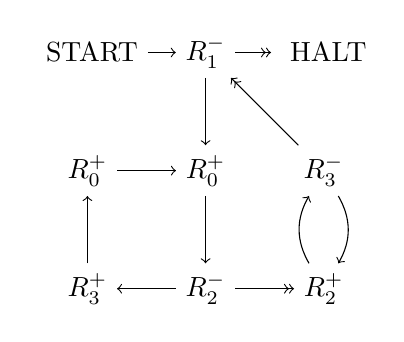
\begin{tikzpicture}[x=1.5cm, y=1.5cm]
                                    \node (s) at (0, 0) {~START~};
                                    \node (l0) at (1, 0) {$R_1^-$};
                                    \node (h) at (2, 0) {~HALT~};
                                    \node (l4) at (0, -1) {$R_0^+$};
                                    \node (l1) at (1, -1) {$R_0^+$};
                                    \node (l6) at (2, -1) {$R_3^-$};
                                    \node (l3) at (0, -2) {$R_3^+$};
                                    \node (l2) at (1, -2) {$R_2^-$};
                                    \node (l5) at (2, -2) {$R_2^+$};
                                    \draw
                                    (s) edge[->] (l0)
                                    (l0) edge[->] (l1)
                                    (l0) edge[->>] (h)
                                    (l1) edge[->] (l2)
                                    (l2) edge[->] (l3)
                                    (l2) edge[->>] (l5)
                                    (l3) edge[->] (l4)
                                    (l4) edge[->] (l1)
                                    (l5) edge[->, bend left=30] (l6)
                                    (l6) edge[->, bend left=30] (l5)
                                    (l6) edge[->>] (l0);
                                \end{tikzpicture}
                            \end{center}
                        \item Give the computation when the register machine is run from the initial configuration $(0, 0, 2, 0, 0)$.
                            \begin{center}
                                \begin{tabular}{ccccc}
                                    $L$ & $R_0$ & $R_1$ & $R_2$ & $R_3$ \\
                                    \hline
                                    0 & 0 & 2 & 0 & 0 \\
                                    1 & 0 & 1 & 0 & 0 \\
                                    2 & 1 & 1 & 0 & 0 \\
                                    5 & 1 & 1 & 0 & 0 \\
                                    6 & 1 & 1 & 1 & 0 \\
                                    0 & 1 & 1 & 1 & 0 \\
                                    1 & 1 & 0 & 1 & 0 \\
                                    2 & 2 & 0 & 1 & 0 \\
                                    3 & 2 & 0 & 0 & 0 \\
                                    4 & 2 & 0 & 0 & 1 \\
                                    1 & 3 & 0 & 0 & 1 \\
                                    2 & 4 & 0 & 0 & 1 \\
                                    5 & 4 & 0 & 0 & 1 \\
                                    6 & 4 & 0 & 1 & 1 \\
                                    5 & 4 & 0 & 1 & 0 \\
                                    6 & 4 & 0 & 2 & 0 \\
                                    0 & 4 & 0 & 2 & 0 \\
                                    7 & 4 & 0 & 2 & 0
                                \end{tabular}
                            \end{center}
                    \end{enumerate}
                \item In this question, you will design register machines that implement subtraction.
                    \begin{enumerate}[(a)]
                        \itemsep0em
                        \item Consider the function $f(x_1, x_2)$ defined as;
                            $$f(x_1, x_2) \triangleq \begin{cases}
                                x_1 - x_2 & \text{if } x_1 \geq x_2 \\
                                0 & \text{otherwise}
                            \end{cases}$$
                            \begin{enumerate}[i.]
                                \itemsep0em
                                \item Define a register machine that computes the function $f$
                                    \begin{align*}
                                        L_0 & : R_2^- \to L_1, L_2 \\
                                        L_1 & : R_1^- \to L_0, L_4 \\
                                        L_2 & : R_1^- \to L_3, L_4 \\
                                        L_3 & : R_0^+ \to L_4 \\
                                        L_4 & : ~HALT~
                                    \end{align*}
                                \item Draw the graph corresponding to the register machine.
                                    \begin{center}
                                        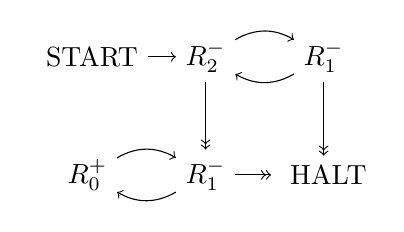
\begin{tikzpicture}[x=1.5cm, y=1.5cm]
                                            \node (s) at (0, 0) {~START~};
                                            \node (l0) at (1, 0) {$R_2^-$};
                                            \node (l1) at (2, 0) {$R_1^-$};
                                            \node (l3) at (0, -1) {$R_0^+$};
                                            \node (l2) at (1, -1) {$R_1^-$};
                                            \node (h) at (2, -1) {~HALT~};
                                            \draw
                                            (s) edge[->] (l0)
                                            (l0) edge[->, bend left=30] (l1)
                                            (l0) edge[->>] (l2)
                                            (l1) edge[->, bend left=30] (l0)
                                            (l1) edge[->>] (h)
                                            (l2) edge[->, bend left=30] (l3)
                                            (l2) edge[->>] (h)
                                            (l3) edge[->, bend left=30] (l2);
                                        \end{tikzpicture}
                                    \end{center}
                            \end{enumerate}
                        \item Consider the partial function $g(x_1, x_2)$ defined as;
                            $$g(x_1, x_2) \triangleq \begin{cases}
                                x_1 - x_2 & \text{if } x_1 \geq x_2 \\
                                \text{undefined} & \text{otherwise}
                            \end{cases}$$
                            \begin{enumerate}[i.]
                                \itemsep0em
                                \item How would a register machine implementing $g(x_1, x_2)$ behave when $x_2 > x_1$?
                                    \medskip

                                    For a register machine to implement $g(x_1, x_2)$, it must halt with $R_0 = y$ when $g(x_1, x_2) = y$.
                                    However, since there is no such $y$, it cannot halt.
                                \item By adapting your answer to part (a), define a register machine that computes the partial function $g$.
                                    \medskip

                                    Since we want the machine to not terminate when $x_2 > x_1$, $L_1$ needs to be modified to cause an infinite loop.
                                    The easiest way to do this is to change $L_1$ to be $L_1 : R_1^- \to L_0, \red{L_1}$, thus cycling back to itself.
                                    \begin{center}
                                        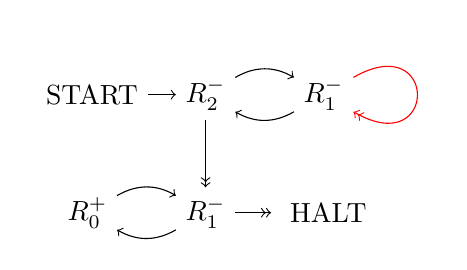
\begin{tikzpicture}[x=1.5cm, y=1.5cm]
                                            \node (s) at (0, 0) {~START~};
                                            \node (l0) at (1, 0) {$R_2^-$};
                                            \node (l1) at (2, 0) {$R_1^-$};
                                            \node (l3) at (0, -1) {$R_0^+$};
                                            \node (l2) at (1, -1) {$R_1^-$};
                                            \node (h) at (2, -1) {~HALT~};
                                            \draw
                                            (s) edge[->] (l0)
                                            (l0) edge[->, bend left=30] (l1)
                                            (l0) edge[->>] (l2)
                                            (l1) edge[->, bend left=30] (l0)
                                            (l1) edge[->>, loop, out=30, in=-30, distance=1.25cm, red] (l1)
                                            (l2) edge[->, bend left=30] (l3)
                                            (l2) edge[->>] (h)
                                            (l3) edge[->, bend left=30] (l2);
                                        \end{tikzpicture}
                                    \end{center}
                            \end{enumerate}
                    \end{enumerate}
                \item Consider the register machine represented by the following graph:
                    \begin{center}
                        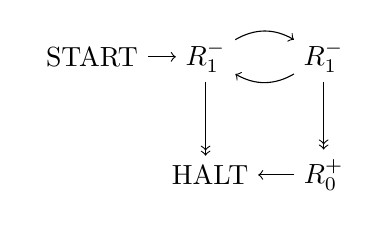
\begin{tikzpicture}[x=1.5cm, y=1.5cm]
                            \node (s) at (0, 0) {~START~};
                            \node (l0) at (1, 0) {$R_1^-$};
                            \node (l1) at (2, 0) {$R_1^-$};
                            \node (l2) at (2, -1) {$R_0^+$};
                            \node (h) at (1, -1) {~HALT~};
                            \draw
                            (s) edge[->] (l0)
                            (l0) edge[->, bend left=30] (l1)
                            (l0) edge[->>] (h)
                            (l1) edge[->, bend left=30] (l0)
                            (l1) edge[->>] (l2)
                            (l2) edge[->] (h);
                        \end{tikzpicture}
                    \end{center}
                    \begin{enumerate}[(a)]
                        \itemsep0em
                        \item Give the code of the register machine.
                            \begin{align*}
                                L_0 & : R_1^- \to L_1, L_3 \\
                                L_1 & : R_1^- \to L_0, L_2 \\
                                L_2 & : R_0^+ \to L_3 \\
                                L_3 & : ~HALT~
                            \end{align*}
                        \item Describe the function of one argument, $f(x)$, that is computed by the register machine.
                            $$f(x) = \begin{cases}
                                1 & x \text{ is odd} \\
                                0 & x \text{ is even}
                            \end{cases}$$
                            Same as computing the remainder of $x$ divided by 2.
                    \end{enumerate}
                \item In order to construct register machines to perform complex operations, it is useful to build them from smaller components that we'll call gadgets, which perform specific operations.
                    \medskip

                    For example, the following gadget tests whether $R_1 = R_2$;
                    \begin{center}
                        \begin{tikzpicture}
                            \draw (0, 0) -- (4, 0) -- (4, -3) -- (0, -3) -- cycle;
                            \node (r1m) at (2, -1) {$R_1^-$};
                            \node (r2ml) at (1, -2) {$R_2^-$};
                            \node (r2mr) at (3, -2) {$R_2^-$};
                            \node (y) at (5, -2) {~yes~};
                            \node (n) at (2, -4) {~no~};
                            \draw
                            (2, 1) edge[->] (r1m)
                            (r1m) edge[->, bend left=30] (r2ml)
                            (r1m) edge[->>] (r2mr)
                            (r2ml) edge[->, bend left=30] (r1m)
                            (r2ml) edge[->>] (n)
                            (r2mr) edge[->] (n)
                            (r2mr) edge[->>] (y);
                        \end{tikzpicture}
                    \end{center}
                    \begin{enumerate}[(a)]
                        \itemsep0em
                        \item Define a gadget "add $R_1$ to $R_2$", which adds the initial value of $R_1$ to register $R_2$, storing the result in $R_2$ but restoring $R_1$ to its initial value (use a scratch register initialised to 0, but must also be reset to 0 after exiting the gadget).
                            \begin{center}
                                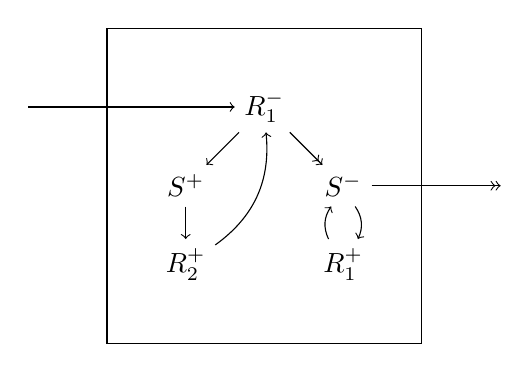
\begin{tikzpicture}
                                    \draw (0, 0) -- (4, 0) -- (4, -4) -- (0, -4) -- cycle;
                                    \node (r1m) at (2, -1) {$R_1^-$};
                                    \node (sp) at (1, -2) {$S^+$};
                                    \node (sm) at (3, -2) {$S^-$};
                                    \node (r2p) at (1, -3) {$R_2^+$};
                                    \node (r1p) at (3, -3) {$R_1^+$};
                                    \draw
                                    (-1, -1) edge[->] (r1m)
                                    (r1m) edge[->] (sp)
                                    (r1m) edge[->>] (sm)
                                    (sp) edge[->] (r2p)
                                    (r2p) edge[->, bend right=30] (r1m)
                                    (sm) edge[->, bend left=30] (r1p)
                                    (sm) edge[->>] (5, -2)
                                    (r1p) edge[->, bend left=30] (sm);
                                \end{tikzpicture}
                            \end{center}
                        \item Define a gadget "copy $R_1$ to $R_2$", which copies the value of $R_1$ into register $R_2$, leaving $R_1$ with its initial value.
                            \begin{center}
                                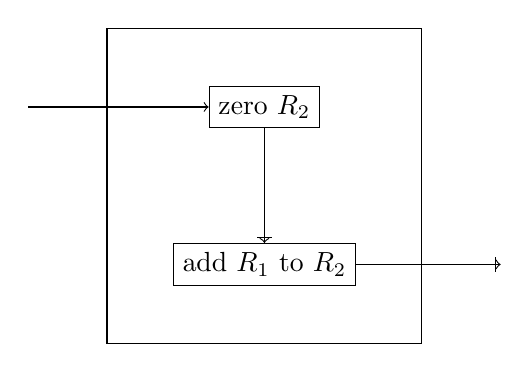
\begin{tikzpicture}
                                    \draw (0, 0) -- (4, 0) -- (4, -4) -- (0, -4) -- cycle;
                                    \node[draw] (zero) at (2, -1) {zero $R_2$};
                                    \node[draw] (add) at (2, -3) {add $R_1$ to $R_2$};
                                    \draw
                                    (-1, -1) edge[->] (zero)
                                    (zero) edge[-|>] (add)
                                    (add) edge[-|>] (5, -3);
                                \end{tikzpicture}
                            \end{center}
                        \item Define a gadget "multiply $R_1$ by $R_2$ to $R_0$", which multiples $R_1$ by $R_2$, and stores the result in $R_0$ (possibly overwriting the initial values).
                            \begin{center}
                                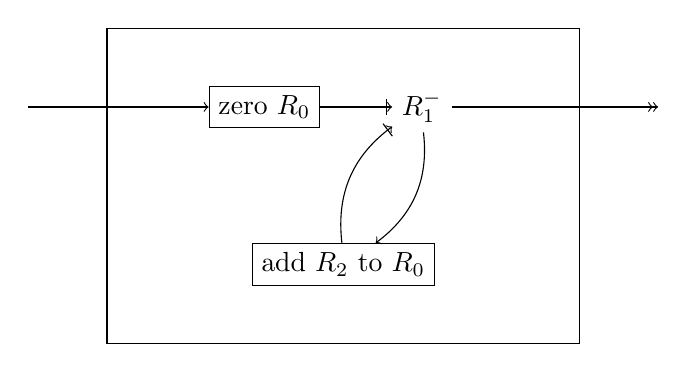
\begin{tikzpicture}
                                    \draw (0, 0) -- (6, 0) -- (6, -4) -- (0, -4) -- cycle;
                                    \node[draw] (zero) at (2, -1) {zero $R_0$};
                                    \node (r1m) at (4, -1) {$R_1^-$};
                                    \node[draw] (add) at (3, -3) {add $R_2$ to $R_0$};
                                    \draw
                                    (-1, -1) edge[->] (zero)
                                    (zero) edge[-|>] (r1m)
                                    (r1m) edge[->, bend left=30] (add)
                                    (r1m) edge[->>] (7, -1)
                                    (add) edge[-|>, bend left=30] (r1m);
                                \end{tikzpicture}
                            \end{center}
                        \item Define a gadget "test $R_1 < R_2$" which determines whether the initial value of $R_1$ is less than that of $R_2$ (possibly overwriting the initial values).
                            \begin{center}
                                \begin{tikzpicture}
                                    \draw (0, 0) -- (4, 0) -- (4, -3) -- (0, -3) -- cycle;
                                    \node (r1m) at (2, -1) {$R_1^-$};
                                    \node (r2ml) at (1, -2) {$R_2^-$};
                                    \node (r2mr) at (3, -2) {$R_2^-$};
                                    \node (y) at (5, -2) {~yes~};
                                    \node (n) at (2, -4) {~no~};
                                    \draw
                                    (2, 1) edge[->] (r1m)
                                    (r1m) edge[->, bend left=30] (r2ml)
                                    (r1m) edge[->>] (r2mr)
                                    (r2ml) edge[->, bend left=30] (r1m)
                                    (r2ml) edge[->>] (n)
                                    (r2mr) edge[->] (y)
                                    (r2mr) edge[->>] (n);
                                \end{tikzpicture}
                            \end{center}
                        \item Describe the function of one argument $f(x)$ computed by the register machine $M$ defined above.
                            \medskip

                            Not really bothered to draw it; starts with $R_2^+$, then to copy $R_2$ to $R_3$, then copy $R_2$ to $R_4$, then multiplies $R_3$ by $R_4$ to $R_6$. copies $R_1$ to $R_5$.
                            It then does a test whether $R_5 < R_6$, if it is, then it halts, otherwise it does $R_0^+$, and goes \textbf{back} to $R_2^+$.
                            \medskip

                            This computes the greatest value $f(x)$ such that $(f(x))^2 \leq x$, hence it computes the floor of the positive square root of $x$.
                            \begin{center}
                                $f(x) = \floor{\sqrt{x}}$
                            \end{center}
                    \end{enumerate}
            \end{enumerate}
\end{document}